% !TeX root = ../main.tex

\chapter{Implementation}\label{chapter:Implementation}

This chapter will discuss, in detail, the added feedback mechanisms and how they were implemented into the \textit{Neurorobotics Unity3D Client}. For the more technical explanations it is assumed the reader has a basic grasp of \gls{cga} and the workings of \textit{Unity3D}.


\section{List of Implemented Feedback Mechanisms}\label{section:feedbackMechanismList}

All listed effects can be disabled or enabled individually, most even at runtime.

\begin{itemize}
    \item \textbf{Interior rendering for objects:} (see \autoref{fig:interiorRendering})
    \newline
    Usually in 3D graphics, only the front facing sides of an object are rendered for performance reasons. The result is that when the camera is inside an object, it will only see the back facing sides of an object, which are not rendered, making them invisible. To correct this, all back facing sides of an object will show the same texture as the front facing sides. The effect of this is that a camera within an object will simply see it inside out, so that a user will be unable to see through walls as easily, and thereby keep his orientation within the object. It is hoped that this will provide a more immersive representation of what being inside of a solid object would look like.
    \newline
    This feedback mechanism is only useful for discrepancies at the head.
    
    \begin{figure}[h]
        \centering
        \subfloat[Interior not rendered]{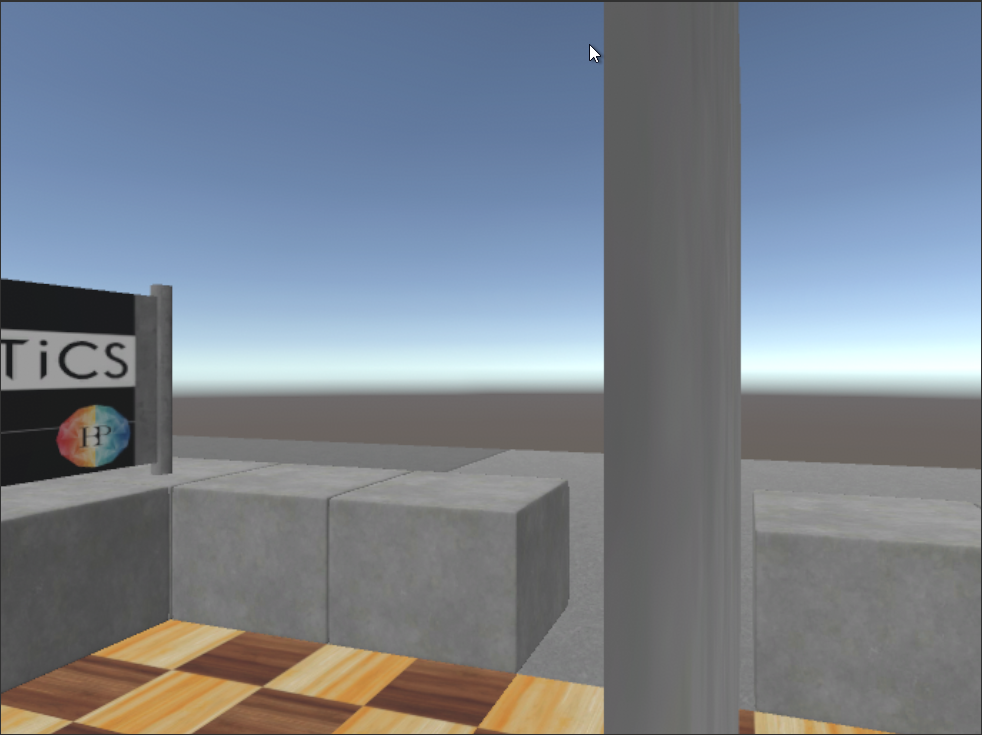
\includegraphics[height=0.2\textheight]{figures/InteriorNotRendered}}
        \hfill
        \subfloat[Interior rendered]{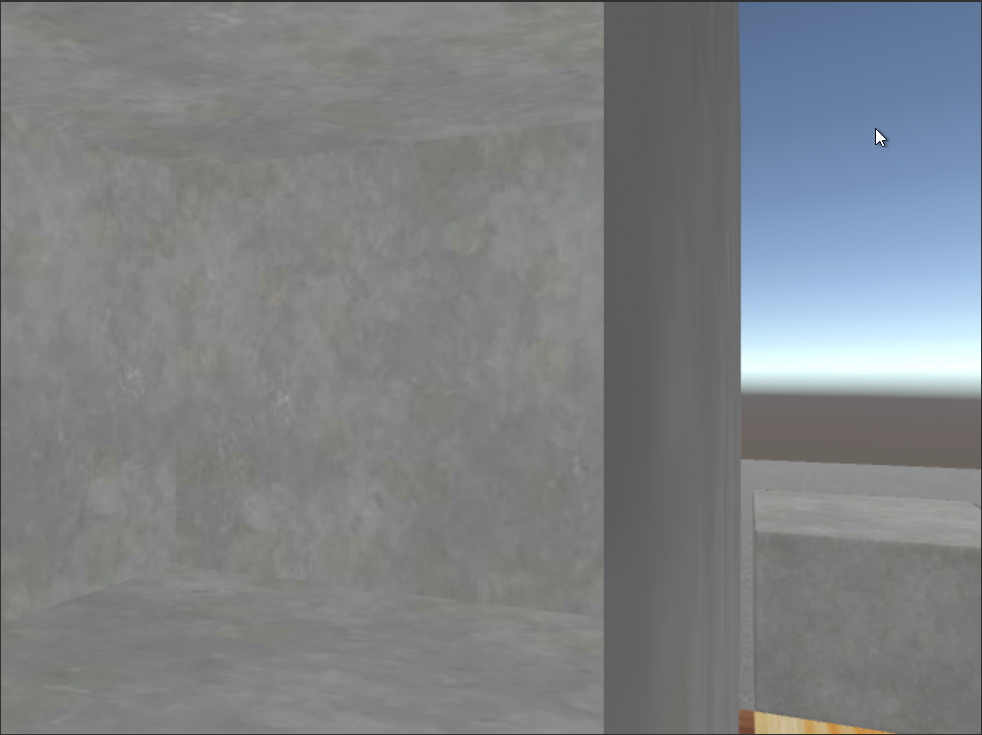
\includegraphics[height=0.2\textheight]{figures/InteriorRendered}}
        \caption{Camera half inside an object. When interior is not rendered, all back facing polygons of the object become invisible}
        \label{fig:interiorRendering}
    \end{figure}
    
    
    \item \textbf{Avatar silhouette visible inside of objects:} (see \autoref{fig:avatarSilhouette})
    \newline
    When the user, for example, steps into an object, the local avatar will follow his tracked foot, however the remote avatar will try to follow, but be stopped from penetrating the object. This will result in the user not being able to see where his real foot is, as he will only see the remote foot in front of the object. Making the silhouette of the local avatar visible, when inside of objects, will allow the user to see exactly where his real body is, while simultaneously seeing where it should be (where the simulated body is).
    \newline
    This should allow the user to keep his orientation as he will never be confused as to where his real limbs are. Due to the way this feature is implemented, the silhouette is only visible as a solid colour. This makes it easy to see when one is inside of an object, but it most likely will have a negative effect on \gls{immersiongl}.
    \newline
    This effect is applied to the entire body and is not dependent on any discrepancies being detected.
    
    \begin{figure}[h]
        \centering
        \subfloat[Avatar silhouette not visible in objects]{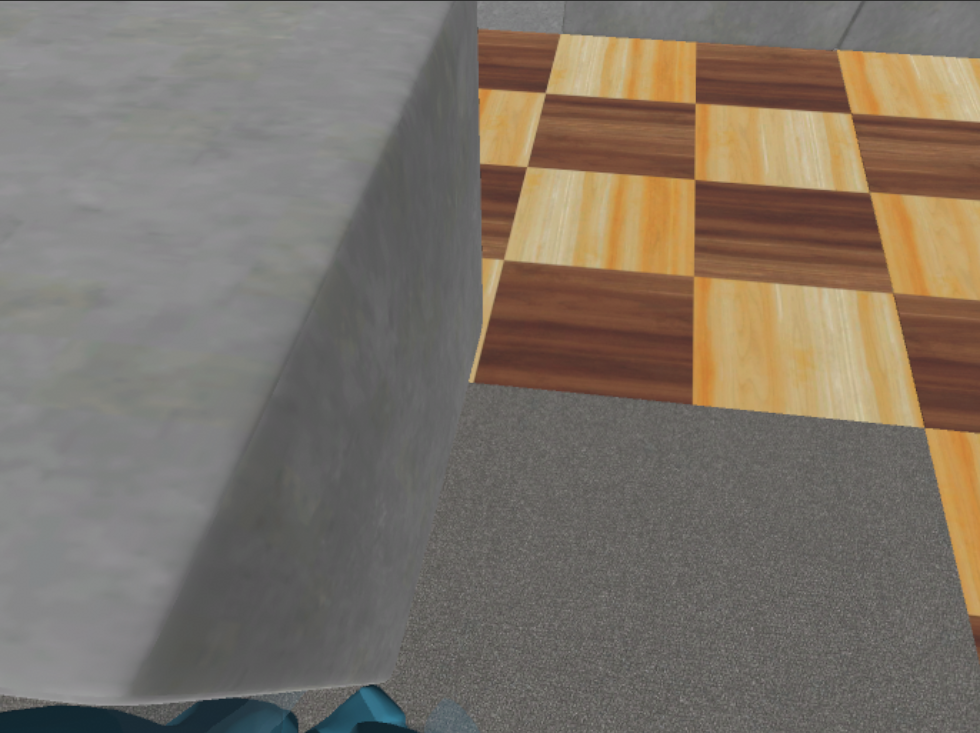
\includegraphics[height=0.2\textheight]{figures/AvatarSilhouetteOff}}
        \hfill
        \subfloat[Avatar silhouette visible in objects]{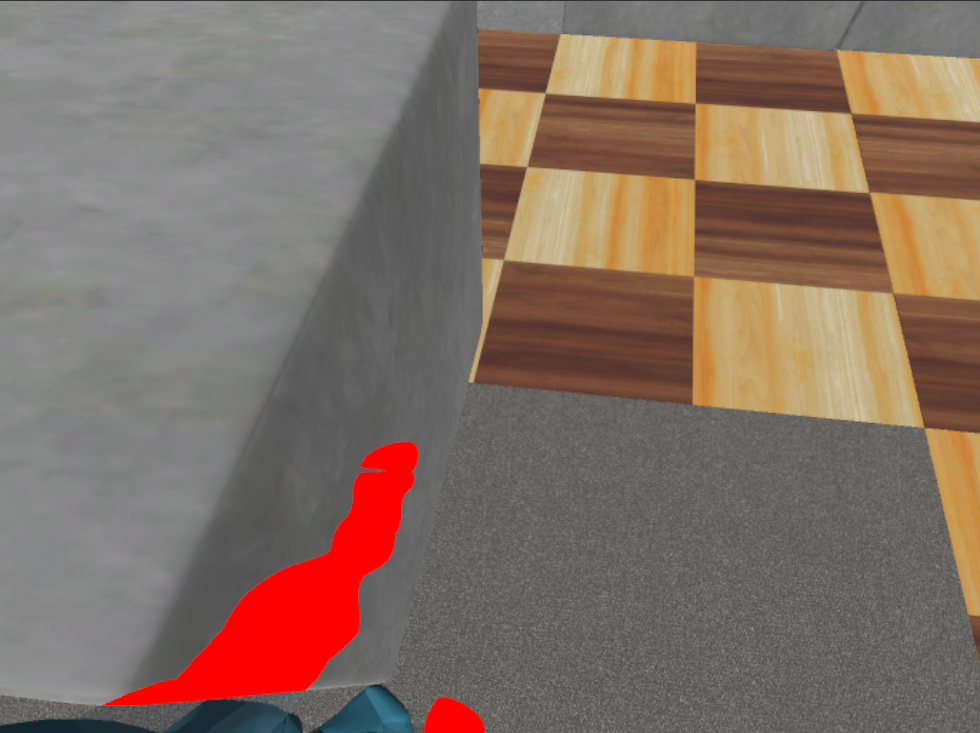
\includegraphics[height=0.2\textheight]{figures/AvatarSilhuetteOn}}
        \caption{Local avatar's left leg partially inside of an object}
        \label{fig:avatarSilhouette}
    \end{figure}
    
    
    \item \textbf{Blur effect:} (see Figure\autoref{fig:blurEffect})
    \newline
    When the head of the local avatar moves away from that of the remote avatar, the user's view will progressively be blurred, for example if his head is inside a low ceiling. This allows the user to keep his orientation, while restricting his view, to alert him to the discrepancy. It should make the user uncomfortable enough to wish to avoid such discrepancies. As blurry vision is something that humans experience in real life, it is anticipated that this effect will have a low impact on \gls{immersiongl}.
    \newline
    This feedback mechanism could also be used for discrepancies at hands and feet, however it was deemed unhelpful during early testing for these purposes, as it restricts the user's view, impeding him from realising where the discrepancy is. It is only used for discrepancies at the head.
    
    \item \textbf{Fade to black effect:} (see Figure\autoref{fig:fadeToBlackEffect})
    \newline
    When the head of the local avatar moves away from that of the remote avatar, the user’s view will progressively fade to black. This is another way of preventing the user from seeing through walls, as he will simply be unable to see anything once the discrepancy is large enough. It has a negative impact on the user's orientation, and should make the user uncomfortable to encourage him to avoid such discrepancies. Vision fading can be likened to humans closing their eyes, and thus this should be a fairly immersive effect.
    \newline
    This mechanism is also possible to use for other discrepancies, but is also deemed unhelpful, like the blur effect. It is only used for discrepancies at the head.
    
    \begin{figure}[h]
        \centering
        \subfloat[Normal view]{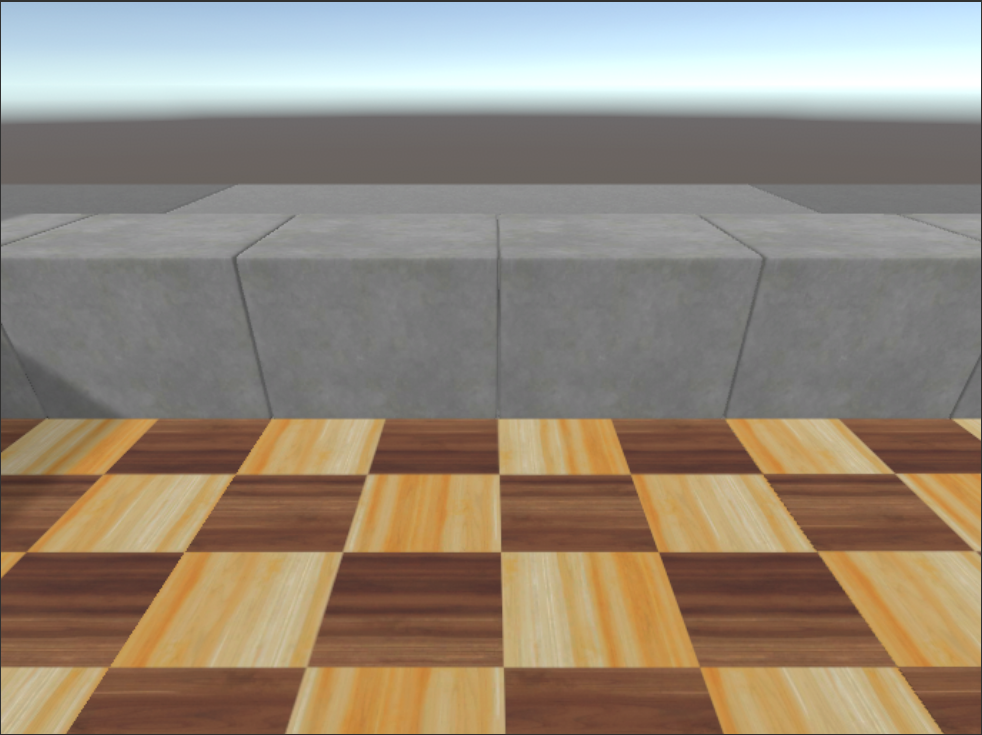
\includegraphics[width=0.3\textwidth]{figures/NoEffects}}
        \hfill
        \subfloat[Blur effect]{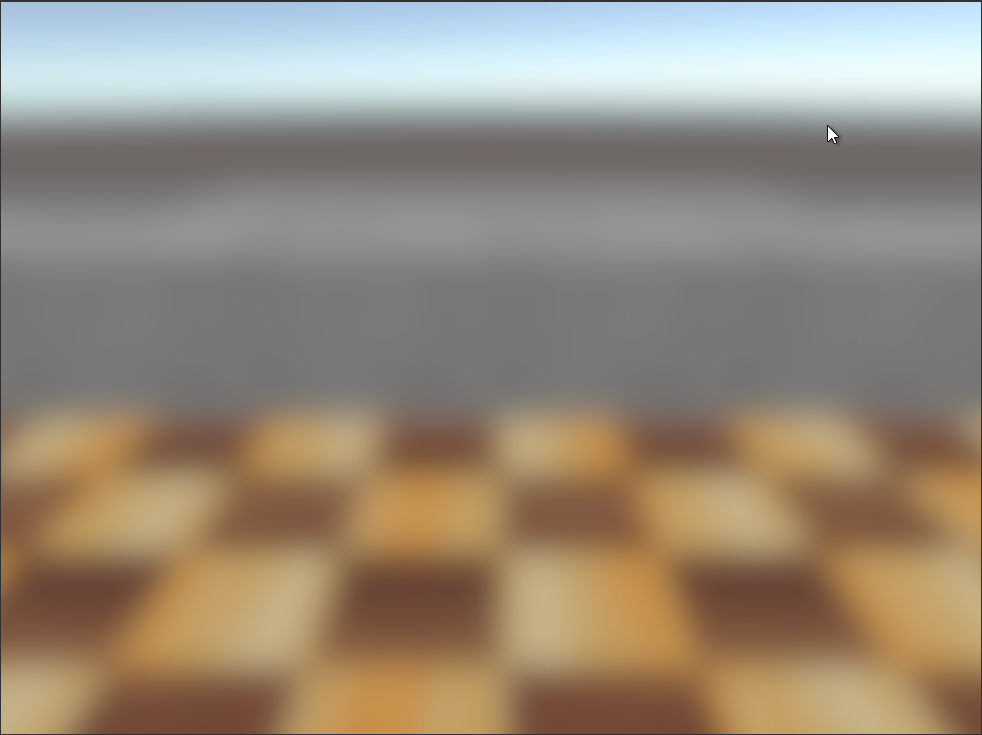
\includegraphics[width=0.3\textwidth]{figures/BlurEffect}\label{fig:blurEffect}}
        \hfill
        \subfloat[Fade to black effect]{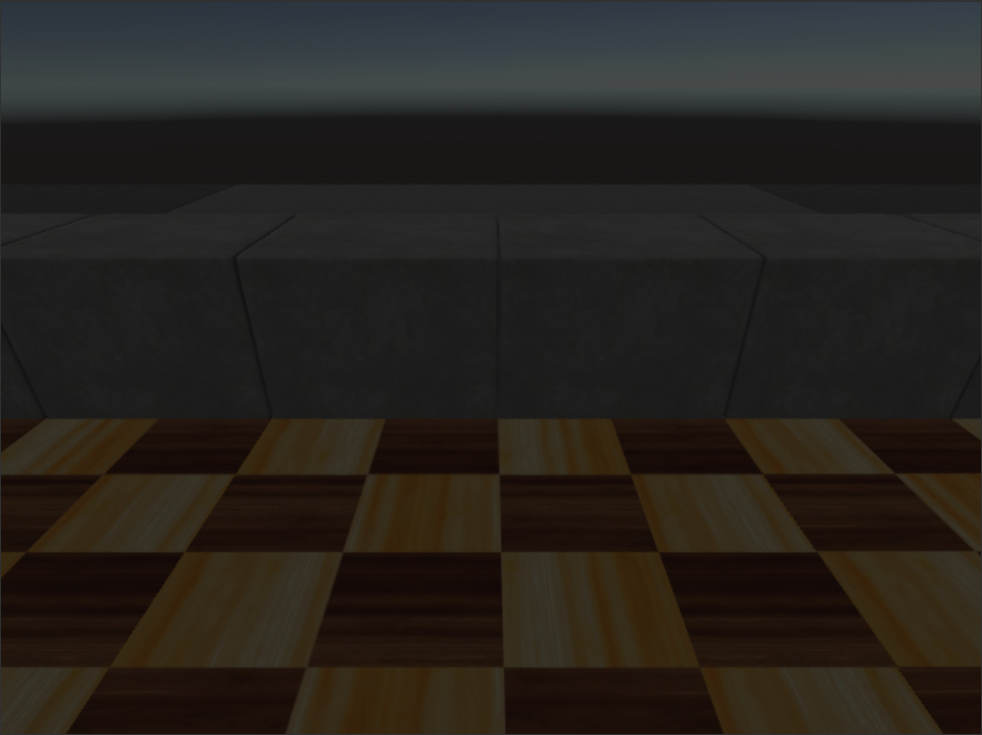
\includegraphics[width=0.3\textwidth]{figures/FadeToBlack}\label{fig:fadeToBlackEffect}}      
        \caption{Blur and Fade to black effects}
        \label{fig:blurFadeToBlack}
    \end{figure}
    
    
    \item \textbf{Line effect:} (see \autoref{fig:LineEffect})
    \newline
    When a local and remote body part (hand or foot) are too far apart, a line is drawn between them, whereby the thickness of the line increases with the distance. The line is thicker on the local end, allowing the user to see which side is which. The main effect of the lines is to show the user which limbs belong together, increasing his sense of orientation towards the remote body. The line effect will probably have a negative impact on \gls{immersiongl}, due to it looking unnatural.
    \newline
    This mechanism also could be used for discrepancies at the head, but there it would not be helpful, since the user can't see the line there anyway. Therefore it is implemented for hands and feet only.
    \begin{figure}[h]
        \centering
        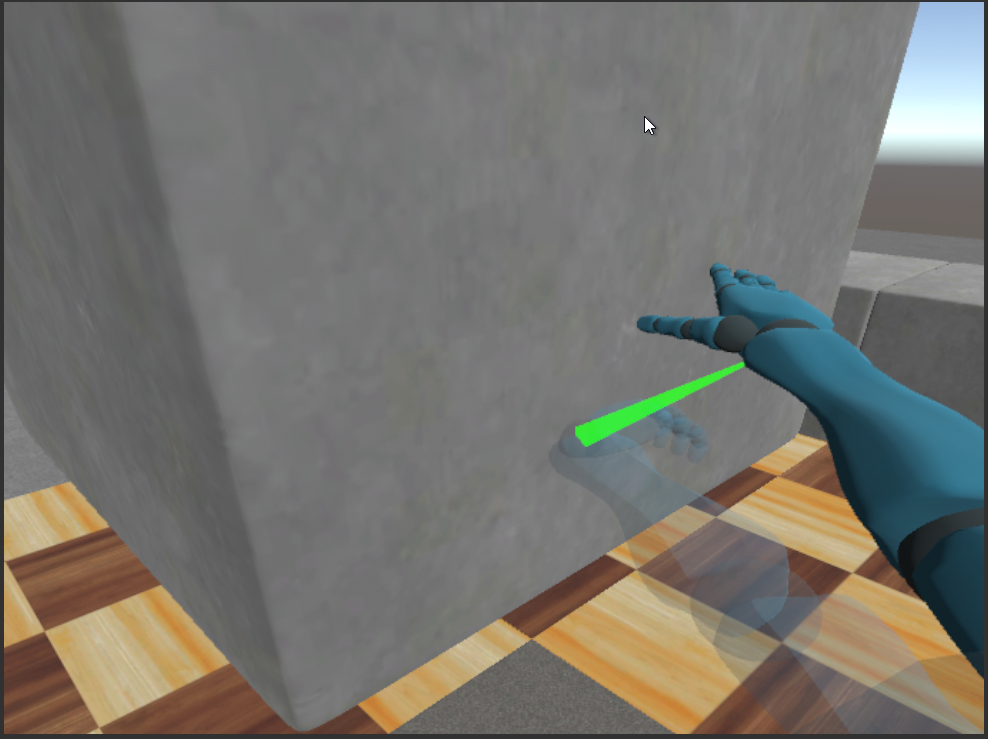
\includegraphics[height=0.2\textheight]{figures/LineEffect.png}
        \caption{Line effect}
        \label{fig:LineEffect}
    \end{figure}
    
    
    \item \textbf{Haptic effect:}
    \newline
    When a discrepancy occurs at a hand, depending on the severity and duration of the discrepancy, the corresponding controller will vibrate in pulses. The duration of one pulse is longer, the larger the discrepancy, and the frequency of pulses increases with increasing duration of the discrepancy. This should give the user an increasing sense of urgency to deal with the discrepancy the larger and longer it is, while being subtle for small and short discrepancies.
    \newline
    Although the \textit{Vive Trackers}, attached to the user's feet, do not have vibration motors of their own, the same vibration instruction can be sent to them, where an external device could be configured to vibrate like the controllers (see \autoref{chapter:Hardware}). This has been implemented, but was not tested due to there currently being no such devices commercially available yet.
    \newline
    Currently this effect only works on discrepancies at the hand.
    
    
    \item \textbf{Geiger sound effect:}
    \newline
    For discrepancies at hands and feet, the Geiger sound effect mimics a Geiger counter, whereby an increase in severity of the discrepancy increases the frequency of clicks. These clicks can be configured to either play from the position of the local or the remote body part. This allows the user to locate the discrepancy without having to see it. The reason for making this effect sound like a Geiger counter is that most people are familiar with its sound as an indicator of danger from video games and movies. It also is a sound based in reality, in order to have a lesser negative effect on \gls{immersiongl}, but is not a pleasant auditory tone, which instils a sense of urgency in the user to deal with this discrepancy.
    \newline
    This effect was not implemented for discrepancies at the head, as the biggest advantage, being able to notice the discrepancy without seeing it, does not apply there.
    
    
    \item \textbf{Noise sound effect:}
    \newline
    Implemented similarly to the Geiger sound effect, this effect simply plays looping static noise from the affected limb when a discrepancy is detected. The volume of this static noise increases with the severity of the discrepancy. As this sound is constant, it is intended to be less distracting than the irregular clicking of the Geiger sound effect.
    
    
    \item \textbf{Discrepancy Indicators:} (see \autoref{fig:discrepancyIndicators})
    \newline
    The discrepancy indicators are little red arrows which rotate around the centre of the user's view to point at a detected discrepancy. It is configurable if these indicators are only visible for discrepancies that are not in the user's view, as well as whether they point at the local or remote limb.
    \newline
    This allows the user to be notified visually of discrepancies not in his view, while also indicating where they are occurring. People not used to \glspl{huda} will probably find these indicators distracting, but people acquainted with \glspl{huda} from video games will probably not experience a negative impact on \gls{immersiongl}.
    This effect was not implemented for discrepancies at the head, as the way the indicators rotate to point to the discrepancies, leads to confusing results, if the discrepancy is very close to the camera, and it was deemed unnecessary to add another visual feedback mechanism for head discrepancies.
    
    \begin{figure}[h]
        \centering
        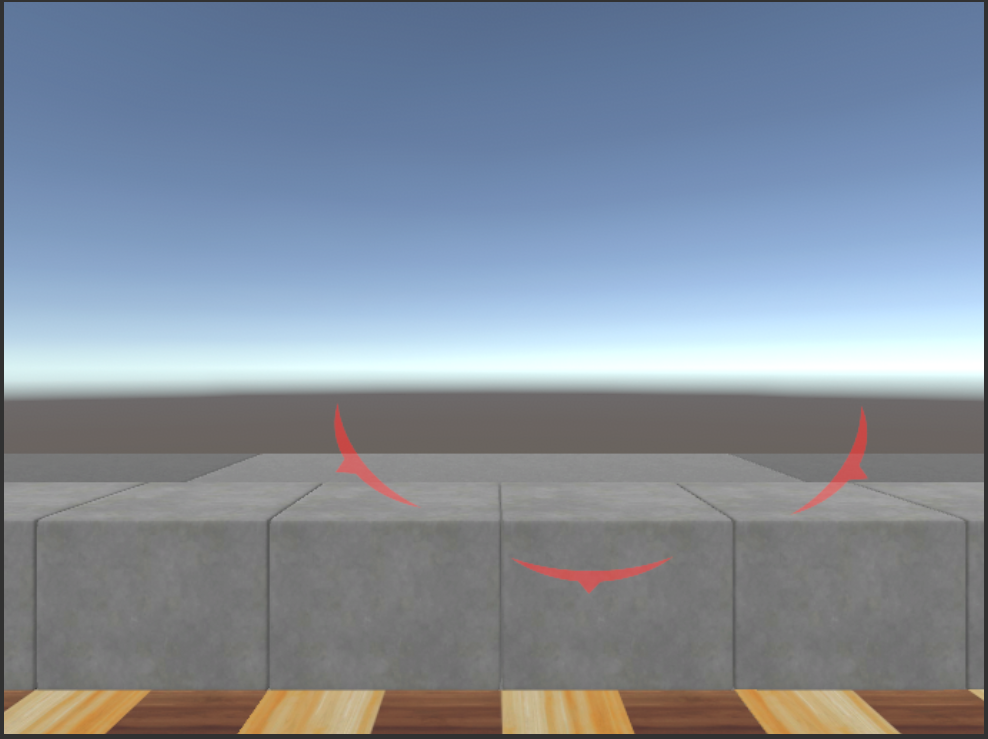
\includegraphics[height=0.2\textheight]{figures/DiscrepancyIndicators.png}
        \caption{Discrepancy indicators pointing at left hand, left foot and right hand}
        \label{fig:discrepancyIndicators}
    \end{figure}


    \item \textbf{Colour shift effect:} (see Figure\autoref{fig:colourShiftEffect})
    \newline
    When a discrepancy is detected, depending on its severity, the hue of all pixels in the user's view is shifted. The effect this has is that colours of all objects change, whereby the change is more drastic, the larger the discrepancy is. It is intended to give the user an increasing sense of there being something wrong, while not inhibiting his vision. Unfortunately, this effect does not indicate where a discrepancy occurs.
    \newline
    This effect is implemented for discrepancies at head, hands and feet, however is probably not as useful, when used universally.
    
    
    \item \textbf{Desaturation effect:} (see Figure\autoref{fig:desaturationEffect})
    \newline
    Similar to the colour shift effect, the desaturation effect lowers the saturation of all pixels in the user's view, depending on the severity of the detected discrepancy. It is more subtle and is used frequently in the context of video games, where it often indicates low health of the player's character.
    \newline
    This effect is implemented for discrepancies at head, hands and feet, however is probably not as useful when used universally.
    
    \begin{figure} [h]
        \centering
        \subfloat[Normal view]{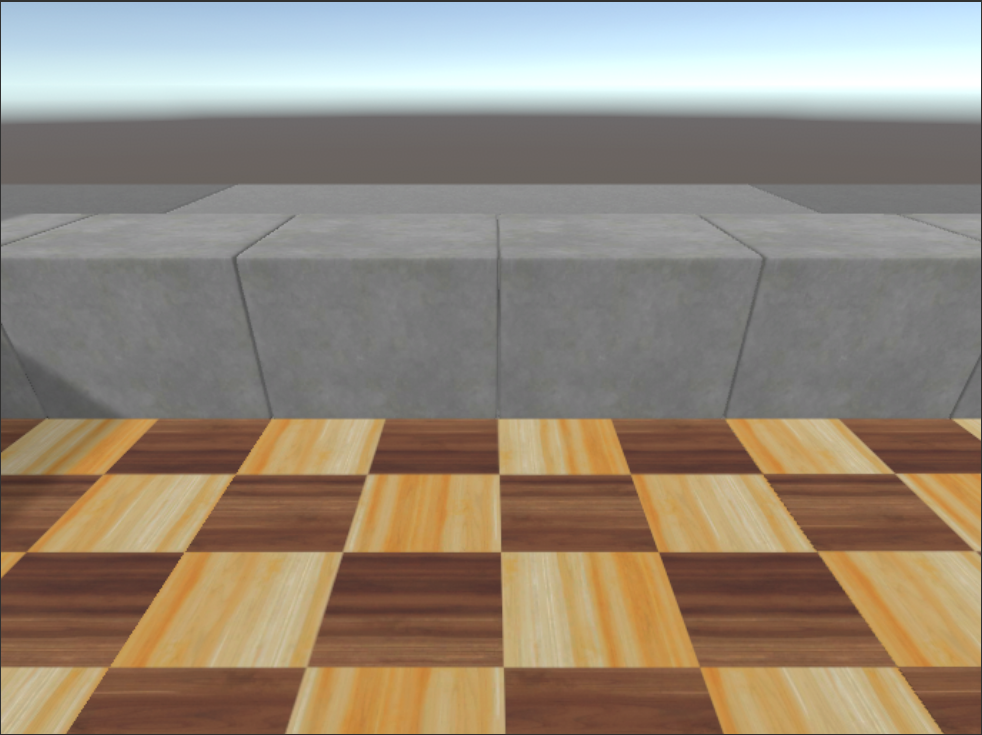
\includegraphics[width=0.3\textwidth]{figures/NoEffects}}
        \hfill
        \subfloat[Colour shift effect]{        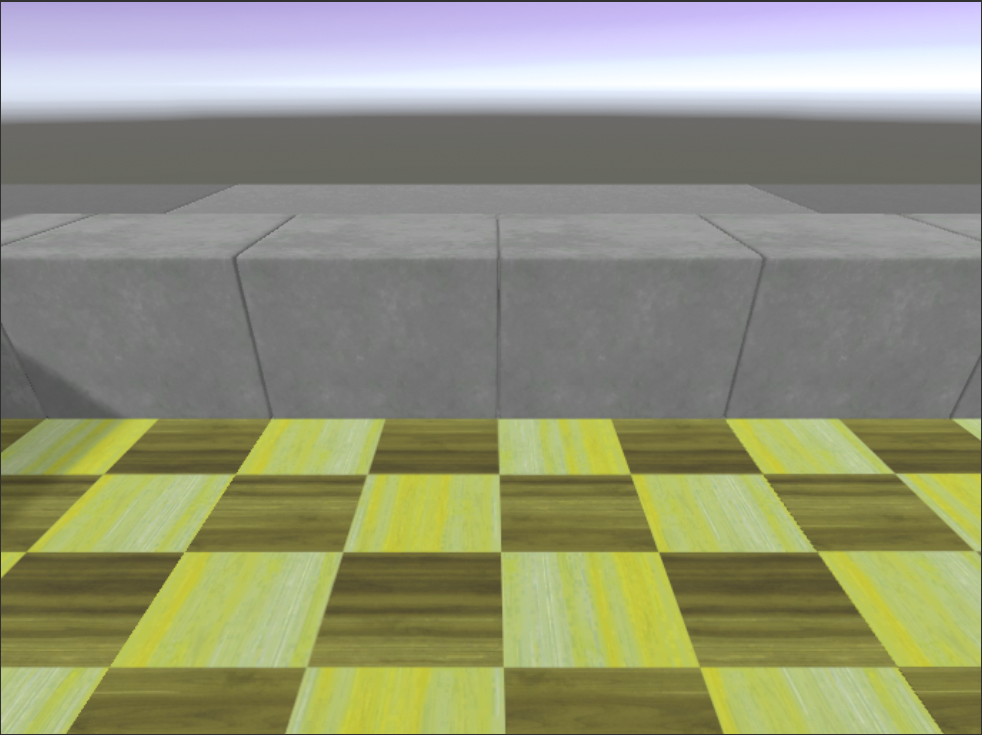
\includegraphics[width=0.3\textwidth]{figures/ColourShiftEffect}\label{fig:colourShiftEffect}}
        \hfill
        \subfloat[Desaturation effect]{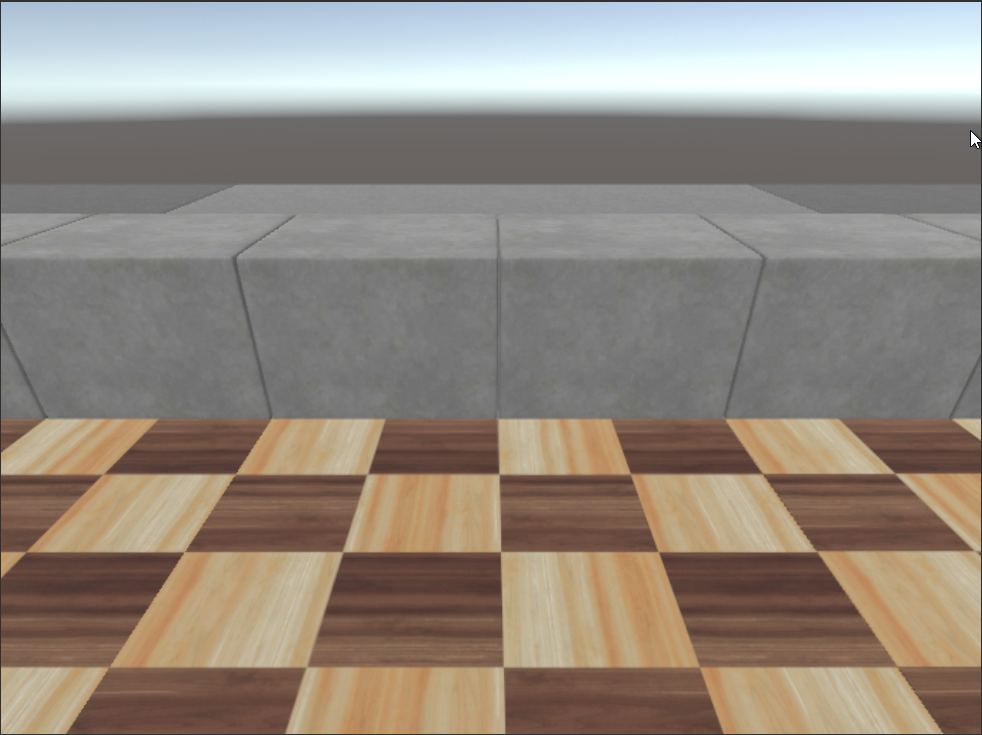
\includegraphics[width=0.3\textwidth]{figures/DesaturationEffect}\label{fig:desaturationEffect}}
        \caption{Normal view, colour shift and desaturation effects}
        \label{fig:normalColourDesaturation}
    \end{figure}
    
    
\end{itemize}


\section{Implementation Details for Feedback Mechanisms}

During the implementation phase, the aim was to create a largely self contained package that could be used in another project with little modification, as well as leaving most existing scripts and functionality of the \textit{Neurorobotics Unity3D Client} unchanged.
All code can be found in the \textit{HBPNeurorobotics/Unity3D-Client} repository in the \textit{VirtualEmbodiment} branch \footnote{\url{https://github.com/HBPNeurorobotics/Unity3D-Client/tree/VirtualEmbodiment},{\newline}mirrored here: \url{https://github.com/VoodaGod/Neurorobotics_Unity3D-Client/tree/VirtualEmbodiment}} in the \texttt{Assets/EmbodimentDiscrepancy} directory.
\newline

The \texttt{DiscrepancyTracker} takes references to the \texttt{Transform} components of all tracked limbs (head, left hand, right hand, left foot, right foot) of the local avatar. Once the remote avatar has been spawned, the corresponding objects to each tracked limb are searched for on the remote avatar. 
\newline
Then, in each frame, the distance between corresponding body parts of the local and remote avatar is computed, and, if greater than a configurable global tolerance, a \texttt{Discrepancy} object is created, which contains the tracked limb, its local position, its remote position, the distance, and the duration of the discrepancy. This object is sent to the \texttt{DiscrepancyHandler}.
\newline

The \texttt{DiscrepancyHandler} contains references to all objects which are responsible for the feedback mechanisms. It also stores the configuration for which effect is enabled for which tracked limb, as well as configurable tolerance timers, before a discrepancy is handled, for each tracked limb.
\newline
For each \texttt{Discrepancy} object sent to it by the \texttt{DiscrepancyTracker} every frame, it is decided which feedback mechanism will be applied for it, based on the configuration. The \texttt{Discrepancy} object is sent on to the designated handler.
\newline
The way these feedback mechanisms are implemented in their handlers will be explained in the following. Apart from the rendering of object interiors and the avatar silhouette inside objects, whose components need to be enabled or disabled before runtime, all effects can be toggled at runtime in the \texttt{DiscrepancyHandler}.


\subsection{Interior rendering for objects}

In order to render the insides of objects, a shader posted on the \textit{Unity} forums by user Tom163\footnote{\url{https://forum.unity.com/threads/what-simple-shader-only-shows-diffuse-without-lighting.41054/\#post-262044}}, which simply displays a texture without any lighting calculations, was adapted to only show the texture on the back facing sides of an object. A material using this shader is added to every object in the \gls{nrpa} scene, except the remote avatar.
\newline
As all \gls{nrpa} objects are created at runtime, the material has to be added to them at runtime as well. In order to do this, the \texttt{modelsParent} variable of the \texttt{GazeboSceneManager} was exposed as a read-only property. It is the parent object of all objects synced from the \gls{nrpa} simulation. For all its child objects with a \texttt{MeshRenderer} component, an instance of the interior material using the same texture as the existing material, is added to the renderer.
\newline 
This is implemented in the \texttt{InteriorRenderingHandler} script.


\subsection{Avatar silhouette visible inside of objects}

In order to make the local avatar visible inside of objects, a shader shown in a \textit{YouTube} video by user N3K EN\footnote{\url{https://www.youtube.com/watch?v=EthjeNeNTsM}} was adapted to only draw a configurable solid colour when an object is between it and the camera. A material using this silhouette shader is added to the local avatar's \texttt{SkinnedMeshRenderers}.
\newline
A problem that arises, is that now the local avatar also constantly shines through the remote avatar. To solve this problem, a stencil test is added to the silhouette shader, whereby no colour is drawn when the configured stencil is set. The remote avatar receives a material using a shader which sets the stencil buffer to the configured value.
\newline
The result is, that if any object is between the camera and the local avatar, the avatar's silhouette will shine through, but not through the remote avatar. This allows the user to still clearly see the remote avatar.
\newline
This is implemented in the \texttt{UserAvatarSilhouetteHandler} script.


\subsection{Blur effect}

The blur effect is implemented in the \texttt{DiscrepancyHeadEffects} script using SuperBlur by user PavelDoGreat\footnote{\url{https://github.com/PavelDoGreat/Super-Blur}}. A \texttt{Discrepancy} object is received from the \texttt{DiscrepancyHandler} in every frame the effect should be active. The intensity of blurring is dependent on the distance of the discrepancy, and the configured \texttt{maxDistToFullBlur}. The amount of blur is smoothly increased when the distance jumps suddenly up from zero, for example when the tolerance timer was reached.


\subsection{Fade to black effect}

This effect is implemented similarly to the blur effect, also in the \texttt{DiscrepancyHeadEffects} script. It uses \textit{SteamVR}'s \texttt{SteamVR\_Fade} functionality, by setting it to black with an increasing alpha value. The amount of darkening is dependent on the configured \texttt{maxDistToBlack} and the distance of the discrepancy. The darkening is also smoothed like in the blur effect.


\subsection{Line effect}

The \texttt{DiscrepancyLineHandler} receives a \texttt{Discrepancy} object from the \texttt{DiscrepancyHandler} in every frame for every tracked limb for which a discrepancy was detected.
\newline
If not existing, a \texttt{DiscrepancyLine} object is created for the tracked limb, and this object draws a line between the local and remote body part, with the thickness of the line depending on the distance of the discrepancy. The thickness can be modified by changing the \texttt{thicknessMultiplier}.
\newline
The appearance of the lines can be changed by adjusting the \texttt{DiscrepancyLinePrefab}.


\subsection{Haptic effect}

\begin{sloppypar}
The haptic effect is implemented in the \texttt{DiscrepancyHapticHandler} script, which has references to \texttt{SteamVR\_TrackedObject}s (the controllers and \textit{Vive Trackers}), which need to be set correctly at run time.
\newline
Every time a discrepancy needs to be handled (also received every frame from the \texttt{DiscrepancyHandler}), the length of the next haptic pulse, as well as the time until the next pulse, is computed for the former by the ratio of distance of the discrepancy to \texttt{maxRumblePulseDistance} and \texttt{maxRumblePulseDuration}, and for the latter by the ratio of duration of the discrepancy to \texttt{maxRumblesTime} and \texttt{maxRumblesPerSecond}. These factors are configurable. To allow for longer vibrations, a coroutine posted by user mptp on the \textit{Steam} forums\footnote{\url{https://steamcommunity.com/app/358720/discussions/0/405693392914144440/\#c357284767229628161}} was adapted.
\newline
The result is longer pulses, the more severe a discrepancy is, and more frequent pulses, the longer a discrepancy has endured.
\end{sloppypar}


\subsection{Geiger sound effect}

This sound effect is implemented in the \texttt{DiscrepancySoundHandler} script. It has a collection of sound clips of Geiger counter clicks, which were taken from a \textit{YouTube} video by user Ryhindor\footnote{\url{https://youtu.be/upPiJ9vOYiY}}. \texttt{Discrepancy} objects are received from the \texttt{DiscrepancyHandler} every frame a discrepancy should be handled. 
\newline
A \texttt{GeigerAudioSourcePrefab} is positioned, as configured, either at the local avatar's limb or the remote avatar's. The intensity of the clicking is calculated with the ratio of distance of the discrepancy to \texttt{geigerDistanceToMaxIntensity} and \texttt{geigerMaxClicksPerMinute}. A random sound clip is played by the corresponding audiosource, as well as the time between clicks being influenced by \texttt{geigerVariance}. 
\newline
The result is more frequent clicking, the larger the discrepancy is. The frequency has some random variance added to make it sound more like a Geiger counter. As the sound is played from either the local or remote limb, the user can identify the position of the discrepancy without seeing it.


\subsection{Noise sound effect}

The noise sound effect is also implemented in the \texttt{DiscrepancySoundHandler}, similarly to the Geiger sound effect. The main difference is that the noise sound, taken from a \textit{YouTube} video by user dalesnale\footnote{\url{https://www.youtube.com/watch?v=8SHf6wmX5MU}}, is continous. Only the volume of the sound is changed, depending on the distance of the discrepancy and \texttt{noiseDistanceToMaxVolume}.
\newline
The result is louder noise coming from either the local or remote limb, the larger the discrepancy.


\subsection{Discrepancy indicators}

The \texttt{DiscrepancyIndicatorHandler} instantiates a \texttt{Canvas} as a child of the main camera. As screen-space canvases are discouraged in \gls{vra} application due to them being hard for the user to focus on, it is a world-space canvas, placed fairly close to the near plane of the main camera.
\newline
On this canvas, for each tracked limb for which a discrepancy needs to be handled, a \texttt{DiscrepancyIndicator} is instantiated. If, in a given frame, a \texttt{Discrepancy} object for a tracked limb is received, the corresponding \texttt{DiscrepancyIndicator} is enabled, and it's rotation set to point, depending on the \texttt{pointsAt} setting, at the local or remote body part.
\newline
When the \texttt{hideIndicatorWhenTargetInView} setting is enabled, the indicator will only be visible, if the target it is pointing to is not in view.


\subsection{Colour shift effect}

\begin{sloppypar}
This effect is implemented in the \texttt{DiscrepancyPostProcessingEffects} script. It uses \textit{Unity3D}'s built in post processing stack. The necessary objects are instantiated at runtime. For all \texttt{Discrepancy} objects received in a frame, the one with the largest distance is used for calculating the amount of colour shift. The amount of shift is also influenced by \texttt{distToFullColorShift} and \texttt{maxShiftDegrees}, whereby shift degrees refers to how far around the colour wheel a colour should be rotated. The calculated value is set in the \texttt{ColorGrading/hueShift} settings of the \texttt{PostProcessProfile}.
\newline
The amount of colour shift is also smoothed for sudden jumps up from zero, for example when the tolerance timer is reached.
\end{sloppypar}


\subsection{Desaturation effect}

\begin{sloppypar}
The Desaturation effect is implemented like the colour shift effect, it just uses the \texttt{ColorGrading/saturation} setting of the \texttt{PostProcessProfile}.
\end{sloppypar}
